\section{Programavimo darbai}

\subsection{Užduotis: Pritaikyti PDF šablonus televizijos paslaugų sutartims}
Šios užduoties aprašymas apima kelias užduotis, kadangi sistemoje yra didelis kiekis skirtingų PDF šablonų,
pavyzdžiui, nauja sutartis, sutarties nutraukimas, paslaugų pajungimas, paslaugų nutraukimas ir t.t.
Klientas pateikė PDF failus, kaip turi atrodyti nauji televizijos sutarčių šablonai (\ref{img:contract} pav.).
Taip pat pakeitimai turi būti pritaikyti ne tik lietuviškoms sutartims, bet ir latviškoms.

\begin{figure}[H]
    \centering
    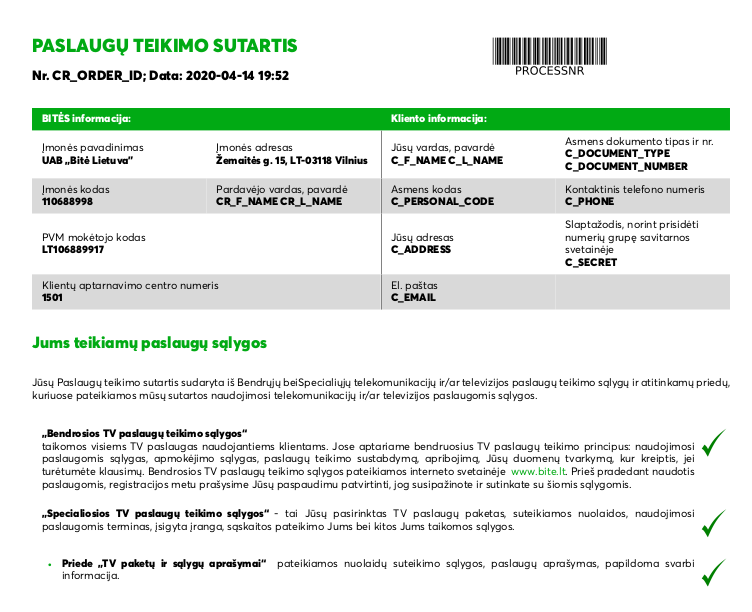
\includegraphics[scale=0.5]{img/contract.png}
    \caption{Naujas televizijos paslaugų PDF šablonas.}
    \label{img:contract}
\end{figure}

\textbf{Problema.} Visi sistemos procesai ir esybės remiasi į mobilųjį numerį (toliau „MSISDN“). Televizijos paslaugos (toliau „TV“) telefono numerio neturi, todėl buvo nuspręsta,
kad pagrindinis TV paslaugų unikalus identifikatorius bus elektroninis paštas (\ref{img:medus} pav.).

\textbf{Analizė.} Telekomunikacijų paslaugų (toliau „GSM“) PDF šablonai yra labai panašūs į TV paslaugų šablonus, tam tikrose vietose vietoj „mobilusis numeris“ pasikeisdavo į
„elektroninis paštas“. Tam tikrose vietose pasikeisdavo statinis tekstas. Tačiau tam tikri šablonai buvo visiškai skirtingi.
Kaip ir buvo minėta, mikroservisų architektūroje kiekvienas servisas atsakingas už tam tikrą funkcionalumą, šiuo atveju, yra du servisai -
vienas atsakingas už lietuviškų sutarčių generavimą, kitas - už latviškų. PDF dokumentų generavimui naudojama „Apache FOP“ „XML“ pagrįsta biblioteka.
„XML“ faile yra aprašomos dokumento formatavimo, stiliaus taisyklės, biblioteka nuskaito iš Java kalbos objekto duomenis, ir juos atvaizduoja nurodytose „XML“ failo vietose.
Taip pat biblioteka palaiko sąlyginius sakinius, ciklus duomenų generavimui.

\textbf{Sprendimas.} Pirminis sprendimas buvo prie PDF dokumento generavimo užklausos objekto pridėti papildomą el. pašto lauką, tačiau šis sprendimas yra gali sukelti klaidų, todėl
jo buvo atsisakyta. Kadangi didžioji dalis sistemos (ne tik PDF dokumentų generavimo) funkcionalumo remiasi į MSISDN lauką, nuspręsta šį lauka pervadinti
į \textit{}„accessPointAddress“, ir jame leisti laikyti elektroninį paštą.
Šis sprendimas nėra pats geriausias, tačiau greičiausias. Šis sprendimas įtakojo PDF dokumentų generavimą, ir tam buvo įvesta žyma
\textit{„contractType“}, kurios reikšmės gali būti arba \textit{„TV“}, arba \textit{„GSM“}.

\textbf{Įgyvendinimas.} Pagal \textit{„contractType“} žymą, atitinkamai buvo generuojama arba TV, arba GSM paslaugų sutartys (\ref{img:contractType} pav.).
Taip pat generuojamiems PDF dokumentams, buvo parašyti parametrizuoti „JUnit“ bibliotekos testai (\ref{img:template} pav.), kurie generuoja skirtingus PDF dokumentus su
skirtingais parametrais (\ref{img:param-tests} pav.), bei tikrina, ar šie duomenys atvaizduojami dokumente.
Tikrinimui naudojami „Hamcrest“ bibliotekos tikrinimo metodai (angl. \textit{„matchers“}).
Tačiau surašius testavimo atvejus, atsirado kita problema - kliento parašas. UI aplikacija, naudojama „Bitė“ salone,
yra prijungta prie planšetinio kompiuterio, kuris, gaudamas žinutę iš aplikacijos, atvaizduoja kliento sutartį, bei leidžia naudojant elektroninį pieštuką, dokumentą pasirašyti.

Parašas buvo įklijuojamas į PDF dokumentą. Problema buvo tame, kad PDF dokumentuose, parašas atsidurdavo ne jam skirtoje vietoje.
Parametrizuoti testai leido anksti atrasti šios problemos egzistavimą, ir atlikus analizę paaiškėjo, kad parašas įklijuojamas pagal šablonui nurodytas koordinates.
Galiausiai problema buvo išspręsta šablonus pakoregavus taip, kad parašo vieta visada liktų toje pačioje vietoje, nepriklausomai nuo duomenų.

\begin{figure}[H]
    \centering
    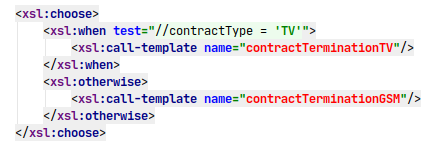
\includegraphics[scale=0.5]{img/contractType.png}
    \caption{\textit{„contractType“} žymos tikrinimas.}
    \label{img:contractType}
\end{figure}

\begin{figure}[H]
    \centering
    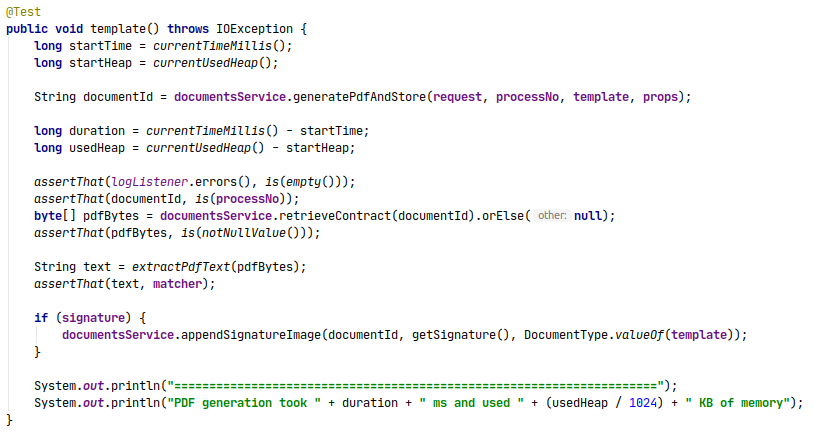
\includegraphics[scale=0.5]{img/template.png}
    \caption{Parametrizuoto testo šablonas.}
    \label{img:template}
\end{figure}

\begin{figure}[H]
    \centering
    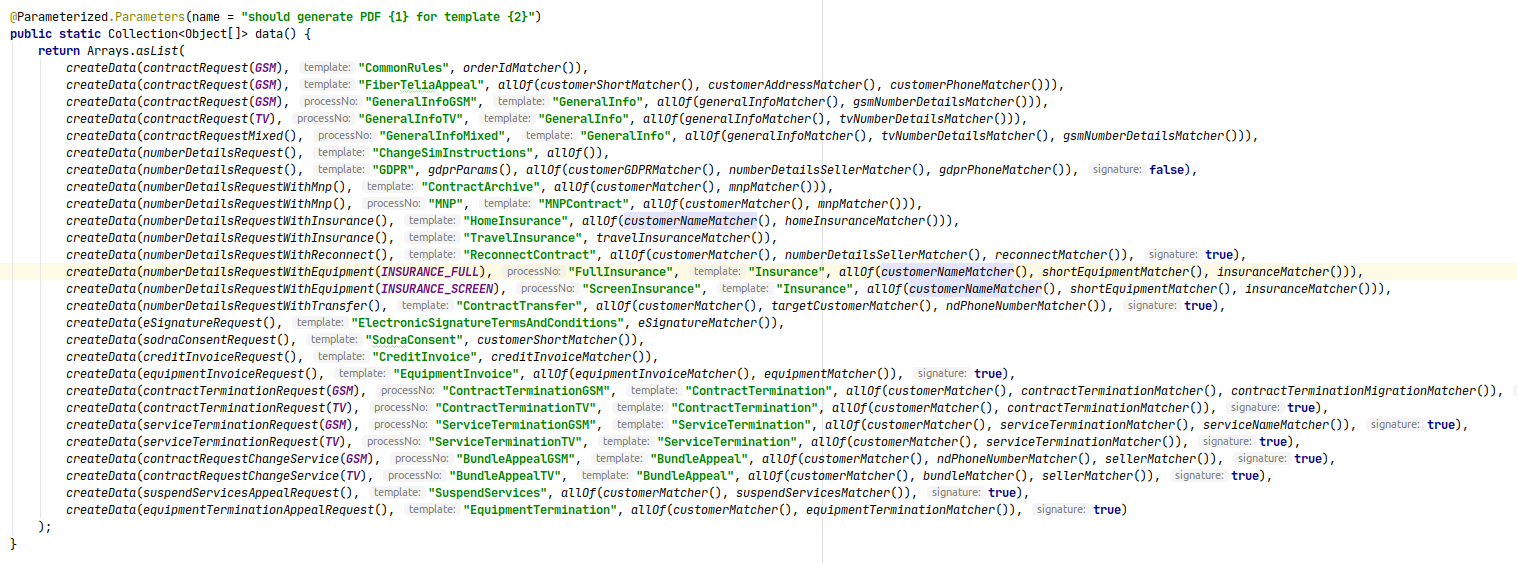
\includegraphics[scale=0.3]{img/param-tests.png}
    \caption{Parametrizuoto testo duomenų sukūrimas.}
    \label{img:param-tests}
\end{figure}


\subsection{Užduotis: El. pašto adreso keitimas.}
\textbf{Problema.} TV sutarties identifikatorius - el. pašto adresas, gali būti keičiamas, tačiau jis turi išlikti unikalus.
Pakeitimas turi būti atvaizduojamas vidinėje apskaitos sistemoje, taip pat UI aplikacijos pakeitimų istorijoje. Keičiant el. pašto adresą, turi būti
atliekamas asinchroninis tikrinimas, ar nurodytas naujas el. pašto adresas yra validus (\ref{img:email-change} pav.).


\begin{figure}[H]
    \centering
    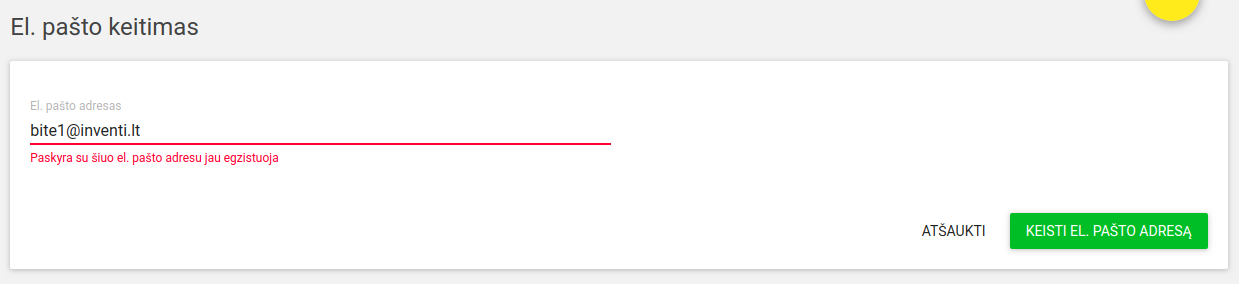
\includegraphics[scale=0.3]{img/email-change.png}
    \caption{El. pašto keitimo procesas.}
    \label{img:email-change}
\end{figure}

\textbf{Analizė.}
Atliekant analizę pastebėta, kad procesas beveik sutampa su „MSISDN“ keitimo procesu, išskyrus validavimo žingsnį, kadangi keičiant „MSISDN“,
vartotojas atlieka paiešką tarp neužimtų „MSISDN“, o el. pašto adresu atveju - adresas įvedamas rankiniu būdu. Pakeitimas turi būti atliktas keliuose servisuose,
taip pat ir UI aplikacijoje. Taip pat pastebėta, kad el. pašto adreso validavimo API yra įgyvendintas, ir naudojamas naujos TV paslaugų sutarties sudarymo metu.

\textbf{Sprendimas.}
Nuspręsta, kad procesas bus įgyvendintas analogiškai, kaip įgyvendintas „MSISDN“ keitimo procesas, išskyrus validavimo žingsnį. Tikrinimui bus naudojamas
egzistuojantis el. pašto adreso validavimo API.

\textbf{Įgyvendinimas.}
Saugomas procedūras įgyvendina „Bitė Lietuva“ programuotojai, reikėjo įgyvendinti šios procedūros kvietimą servise, kuris sąveikauja su apskaitos sistemos duomenų baze.
Buvo įgyvendintas SOAP protokolo API, kurio kvietimui buvo atnaujintas kitas servisas, atsakingas už REST užklausų vertimą į SOAP. Šio serviso API kvietimas įgyvendintas
kitame servise, kuris glaudžiai bendrauja su UI aplikacija. Šiame servise taip pat įgyvendintas el. pašto validavimas, tam kad vartotojas negalėtų apeiti šį žingsnį,
nenaudodamas aplikacijos UI. El. pašto adreso validavimo žingsnis buvo įgyvendintas tiek sinchroniškai, tiek asinchroniškai (\ref{img:email-validate} pav.).
Sudėtingumas iškilo atlikus el. pašto validavimo API. API įgyvendintas naudojant „Apache Camel“ technologiją, su kurią patirties neturėjau.
Naujos paslaugų sutarties sudarymo metu, el. pašto validavimo API reikalauja kitų duomenų iš užsakymų krepšelio, kurių el. pašto keitimo proceso metu, nėra.
Taip pat servisas, API kvietimo metu, iškviečia 5 skirtingų servisų API, tam kad užtikrinti el. pašto unikalumą. Jeigu bent vienas API grąžina klaidą, vartotojui grąžinamas
klaidos kodas, o UI aplikacijoje pagal klaidos kodą parenkamas vertimas.

\begin{figure}[H]
    \centering
    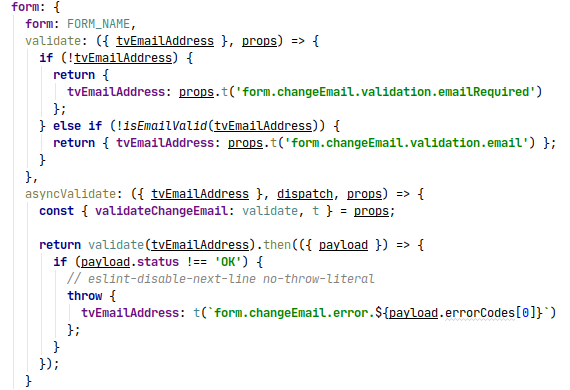
\includegraphics[scale=0.7]{img/email-validate.png}
    \caption{„React“ komponento el. pašto keitimo validavimo kodas.}
    \label{img:email-validate}
\end{figure}

El. pašto keitimo metu, tam tikros validacijos nėra būtinos, todėl nuspręsta validavimo API perduoti el. pašto validavimo proceso tipą, pagal kurį servisas nusprendžia,
kuriuos kvietimus būtina atlikti.


\subsection{Užduotis: Krepšelio REST API dokumentacija.}

\textbf{Problema.}
Kaip buvo minėta ankščiau, dauguma sistemos procesų vykdomi per krepšelį, nurodant proceso pavadinimą. Sistemoje galima pridėti skirtingas paslaugas į krepšelį,
pašalinti iš krepšelio, tačiau svarbiausias žingsnis - krepšelio tvirtinimas (angl. \textit{„checkout“}). Šis žingsnis reiškia, kad krepšelio duomenys perduodami kitam servisui sutarties
generavimui. Tačiau pardavimus planuojama vykdyti ne tik per „medus“ sistemą, „Bitė Lietuva“ programuotojų komanda vykdo savitarnos kūrimo projektą „Go3 | BITĖ“, leidžianti
klientui savarankiškai užsisakyti paslaugas. Šiam funkcionalumui įgyvendinti buvo sukurtas krepšelio tvirtinimo REST API, kuriam perduodant duomenis, paslaugos galėtų būti aktyvuotos
be UI aplikacijos pagalbos. Kadangi REST API įgyvendino „INVENTI“ programuotojai, šios užduoties tikslas - suteikti informaciją apie API, padėti „Bitė Lietuva“ sukurti integraciją.

\textbf{Analizė.}
Analizę sudarė informacijos apie REST API laukus rinkimas. Pagrindiniai informacijos šaltiniai - komandos nariai, turintys patirties dirbant su šia sistema,
taip pat „Bitė Lietuva“ darbuotojai - sistemos analitikai.

\textbf{Sprendimas.}
Nuspręsta REST API dokumentaciją sudaryti naudojant \textit{„Swagger 2“} biblioteką. Ši biblioteka leidžia nesudėtingai, anotacijų pagalba, dokumentuoti sistemos REST API.
Biblioteka yra lengvai konfigūruojama, taip pat yra galimybė sukonfigūruoti \textit{„Swagger UI“} (\ref{img:swagger} pav.\footnotemark[4]) sąsają,
kuri leidžia atlikti REST API operacijas, ir yra pasiekiama  per nuorodą. Taip pat ši biblioteka leidžia REST API duomenis pasiekti JSON formatu, dėl šios priežasties,
yra galimybė importuoti API dokumentaciją ir naudotis kitais įrankiais, pavyzdžiui, \textit{„Postman“}.

\footnotetext[4]{Paimta iš oficialaus \textit{„swagger.io“} puslapio.}

\begin{figure}[H]
    \centering
    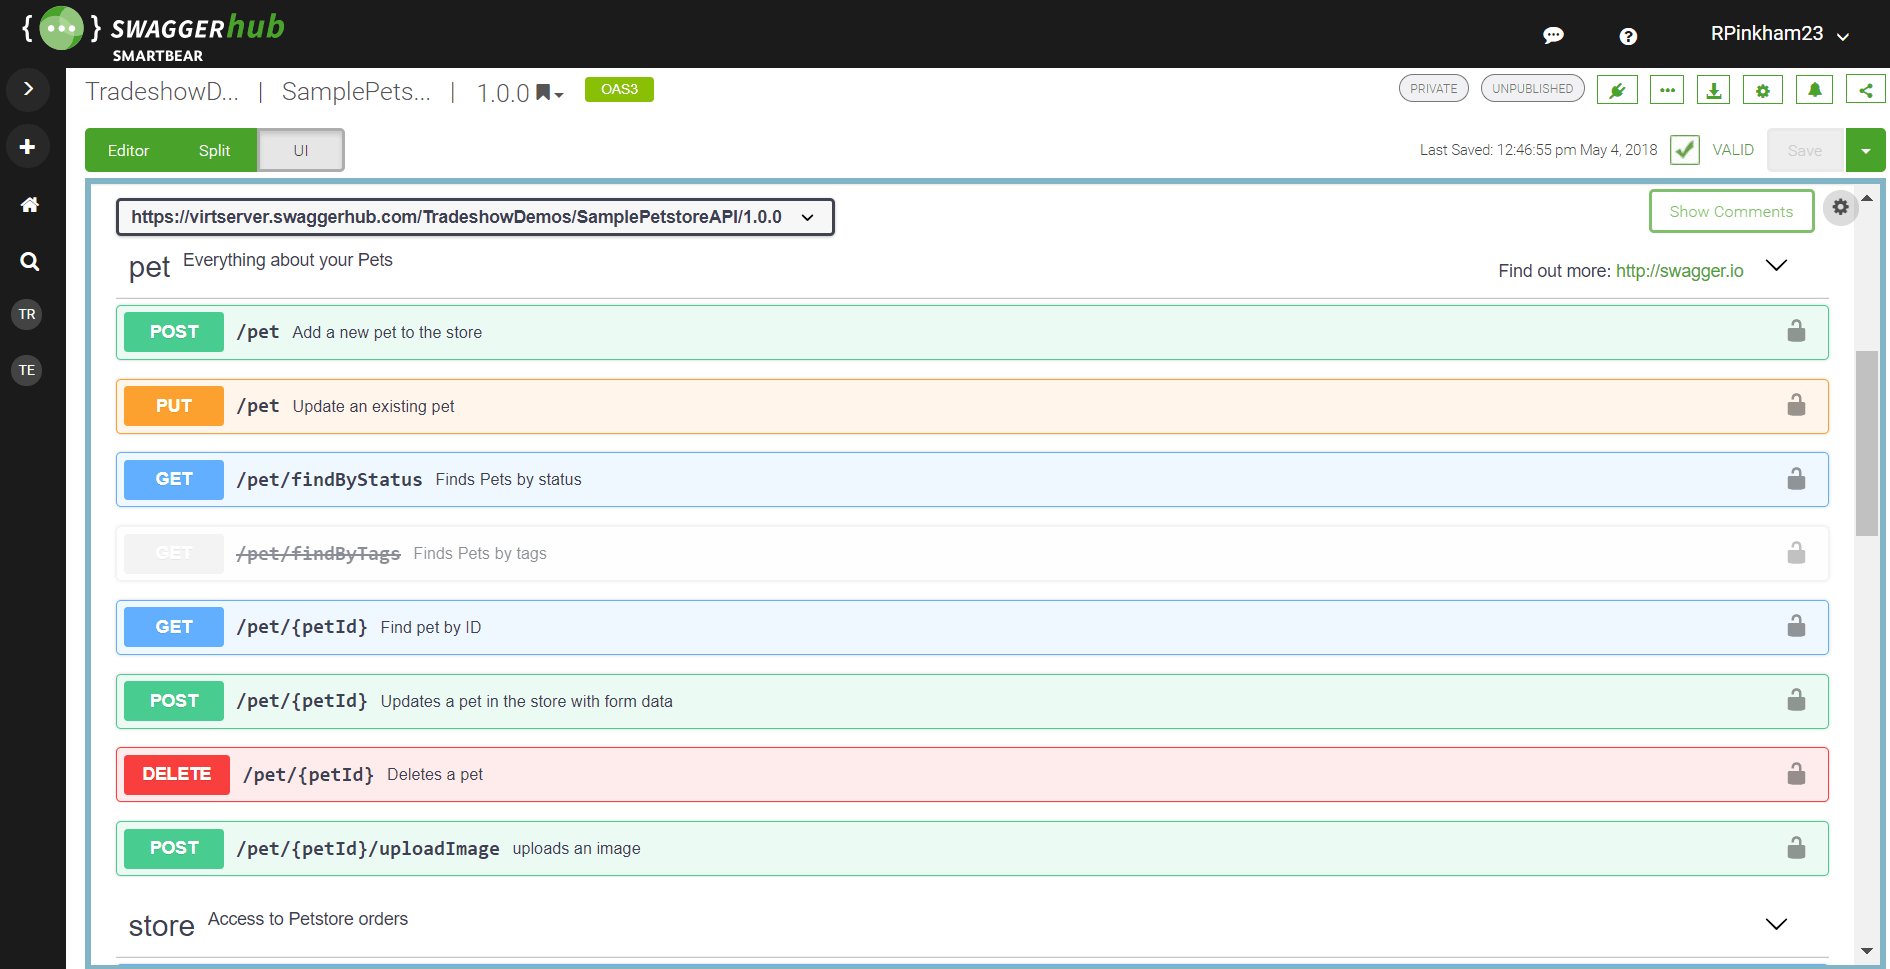
\includegraphics[scale=0.25]{img/swagger.png}
    \caption{„Swagger UI“ sąsaja.}
    \label{img:swagger}
\end{figure}

\textbf{Įgyvendinimas.}
Apibrėžtiems REST API užklausos laukams buvo sudėtos anotacijos, kurioje nurodoma, už ką laukas atsakingas, taip pat pateikiami pavyzdžiai (\ref{img:customer-dto} pav.).
Tačiau šio API problema tame, kad didžioji dalis laukų yra neprivalomi. Dėl šios priežasties, šie laukai nėra apibrėžti kode, o sudedami į \textit{„Map“} duomenų struktūrą, iš kurios
vėliau ištraukiami pagal raktą. Tačiau \textit{„Swagger 2“} leidžia apibrėžti savo duomenų tipą, ir jį priskirti bet kuriam laukui. Atlikus detalesnę kodo analizę, pavyko surinkti
visas įmanomas šios duomenų struktūros reikšmes, kurios vėliau buvo dokumentuojamos.
\textit{„Bitė Lietuva“} programuotojų komandai pora kartų kilo problemos su šiuo REST API, tačiau pateikus užklausos pavyzdį, klaidos buvo greitai identifikuotos ir pašalintos.


\begin{figure}[H]
    \centering
    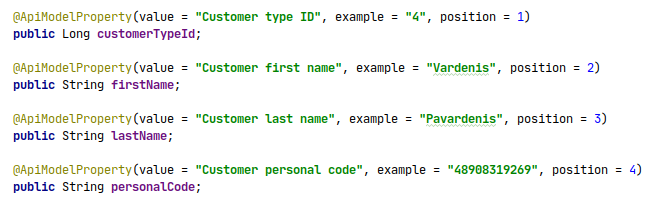
\includegraphics[scale=0.5]{img/customer-dto.png}
    \caption{\textit{„Swagger 2“} dokumentavimo pavyzdys.}
    \label{img:customer-dto}
\end{figure}
